%!TEX root = thesis.tex

\chapter{Evaluation}
\label{chapter:evaluation}

In this chapter, we describe the evaluation of the tool built. The evaluation is performed by using two separate methods: we evaluate the efficiency of development process with the software effort and complexity metrics presented in chapter \ref{chapter:methods}, and visualization effectiveness with guidelines by \citet{kraak_cartographic_1998} complemented by visualization heuristics by \citet{zuk_heuristics_2006} and map objectives by \citet{schlichtmann_visualization_2002} presented in chapter \ref{section:visualizationprinciples}. As using either of the methods requires a baseline project, we decided to implement a number of sister projects as defined by \citet{kitchenham_evaluating_1998}. In this chapter, the visualizations built during sister projects are referred to with the term ``reference visualization'' while the visualizations built with Thematic.js are referred to with ``Thematic.js visualization''. \fixme{Are these terms clear enough?}

\section{Defining the Evaluated Cases}

The visualization tool should be able to visualize a large variety of data. Moreover, the benefits of reusable software are typically emphasized when examining a large number of relatively similar cases \citep{frakes_software_1996}. However, in order to keep the scope of this work manageable, we decided to evaluate a set of visualization cases listed below.

\paragraph{Alko stores in Finland}
Store locations are most naturally visualized using a dot map. Alko provides an unsupported representational state transfer (REST) API\footnote{\url{http://www.alko.fi/api/store/mapmarkers?language=fi}} for fetching data of Alko stores. The data is in a non-standard ``flat dot'' format (see appendix \ref{appendix:flatdotformat}). We decided to visualize locations using a dot map. This case is later referred to as ``store map''.

\paragraph{Earthquakes in California}
Earthquakes have two fundamental data axes: location and magnitude. Therefore, earthquakes are best visualized using a proportional symbol map with the size of the symbol representing magnitude. United States Geological Survey provides historical earthquake data\footnote{\url{http://earthquake.usgs.gov/earthquakes/search/}}, and we decided to visualize earthquakes in California since January 1, 1900. The data is available in a Comma-Separated Values (CSV) format which is can be trivially transformed to ``flat dot'' JSON format. This case is later referred to as ``earthquake map''.

\paragraph{Circulation of the Biggest Finnish Newspapers}
\fixme{Describe this}

\paragraph{Voter Turnout in Finnish Presidential Election of 2012}
The Finnish Ministry of Interior provides regional voter turnout data of the presidential election of 2012\footnote{\url{http://tulospalvelu.vaalit.fi/TP2012K2/s/aanaktiivisuus/aanestys1.htm}}. This data is provided in electoral district and municipality level. We decided to visualize the turnout in municipality level, using municipality data by the Finnish Land Survey\footnote{\url{http://www.maanmittauslaitos.fi/en/opendata}}. The municipality data is provided in GeoJSON format by Teemu Tiilikainen\footnote{\url{https://github.com/varmais/maakunnat}}. These data can be combined to create an effective choropleth visualization of regional turnout. The data should be normalized in quantized fashion, i.e., using thresholds to create a discrete color range. This case is later referred to as ``election map''.

\paragraph{Share of People with No Secondary Education in Finland}
Statistics Finland\footnote{\url{http://www.tilastokeskus.fi/}} provides provincial data on the education of the population of Finland in CSV format. This can be combined with province data by the Finnish Land Survey\footnote{\url{http://www.maanmittauslaitos.fi/en/opendata}} to create an effective choropleth visualization. The data should be normalized in linear fashion, i.e., using continuous color range. This case is later referred to as ``education map''.

\paragraph{Travel Times to a Single Destination}
Travel times to a destination can be visualized using an isarithmic map. We decided to visualize travel times to Futurice headquarters\footnote{\url{http://futurice.com/contact\#helsinki}} using public transport. The travel times can be obtained by using Travel Time Visualization Utility for HSL Reittiopas\footnote{\url{https://github.com/pyryk/reittiopas-travel-times}} which provides the data in an approximated ``flat dot'' format. The data should be normalized in a quantized fashion to emphasize isarithmic contours. This case is later referred to as ``simple travel times map''.

\paragraph{Travel Times to Multiple Destinations}
In addition to visualizing travel times to a single destination, we decided to evaluate a case for displaying travel times to multiple destinations. The travel times are obtained with the method defined in the previous paragraph, and combined using a weighted average method. Like in the previous case, the data should be normalized in a quantized fashion. This case is later referred to as ``complex travel times map''.

\fixme{Add dasymetric? Then would cover all methods}

~

While the visualized data is arbitrarily selected, the cases are picked to reflect the typical usage of visualizations. Choropleth map and isarithmic map are the most frequenly used thematic mapping methods \citep[chap.~14-15]{slocum_thematic_2014} and therefore it is beneficial to the evaluation to examine multiple visualizations with those methods.

In order to better model typical real-life use cases, and to be usable on the web, the visualization cases include also a generic application structure and HTML features \fixme{such as...} which are required for web applications.

\section{Implementing Sister Projects}

We implemented seven separate sister project visualizations with no visualization library to compare to visualization cases as defined in the previous section. The functionality of the visualizations was designed to reflect the functionality of the evaluated visualizations as accurately as possible. Sister visualizations were implemented using HTML, CSS and JavaScript to enable straightforward comparison to the evaluated visualization cases. While we did not use any visualization library for the sister projects, we deemed using a generic mapping library such as Leaflet.js appropriate, because typically, creating map visualizations is not feasible without using one. Moreover, also Thematic.js uses Leaflet.js as a mapping library.

In order to better reflect the actual situations involving building visualizations, the sister projects were implemented in \emph{ad hoc} fashion, meaning that the design or architecture of the applications were not planned extensively beforehand. Also, no reuse of any form between visualizations was planned. However, during implementation, some design and code scavenging was done in order to speed up the development process.

\section{Evaluating Efficiency of Development}

We evaluated the efficiency of development by several metrics: software code length (number of physical (LOC) and logical (LLOC) lines of code), cyclomatic complexity (CC), Halstead difficulty (HD) and Halstead effort (HE). For measurements, we used ESComplex\footnote{\url{https://github.com/philbooth/escomplex}} for analyzing JavaScript programs. \fixme{What about HTML and CSS? Any way to measure these? Or is the effort for these considered equal in sister projects?}

We began the evaluation by measuring the aforementioned metrics for the visualizations. It should be noted that for these measurements, we did not include code from Thematic.js or other third party libraries. The measurements are shown in table \ref{table:efficiencymetrics}.

~

\LTcapwidth=\textwidth
\begin{longtable}{|l|c|c|c|c|c|}
\hline
\textbf{Visualization} & \textbf{LOC} & \textbf{LLOC} & \textbf{CC} & \textbf{HD} & \textbf{HE} \\ 
\hline
Thematic.js store & 12 & 12 & 1 & 7.31 & 4600 \\
Reference store & 126 & 85 & 10 & 23.6 & 96500 \\
Thematic.js earthquake & 15 & 14 & 1 & 8.38 & 6280 \\
Reference earthquake & 79 & 121 & 10 & 23.5 & 87400 \\
Thematic.js election & 26 & 29 & 2 & 10.9 & 12800 \\
Reference election & 141 & 101 & 14 & 23.8 & 107000 \\
Thematic.js education & 17 & 17 & 1 & 10.2 & 10200 \\
Reference education & 129 & 87 & 10 & 27.8 & 109000 \\
Thematic.js travel times simple & 27 & 28 & 2 & 10.8 & 9840 \\
Reference travel times simple & 184 & 129 & 12 & 29.4 & 182000 \\
Thematic.js travel times complex & 30 & 30 & 2 & 11.6 & 13300 \\
Reference travel times complex & 193 & 144 & 12 & 34.5 & 255000 \\
\hline
\caption{Measurements for developed visualizations, including only visualization-specific code. \fixme{Complete the table with real data} \fixme{Add the last missing visualization}}
\label{table:efficiencymetrics}
\end{longtable}

\begin{figure}[htbp]
  \begin{center}
    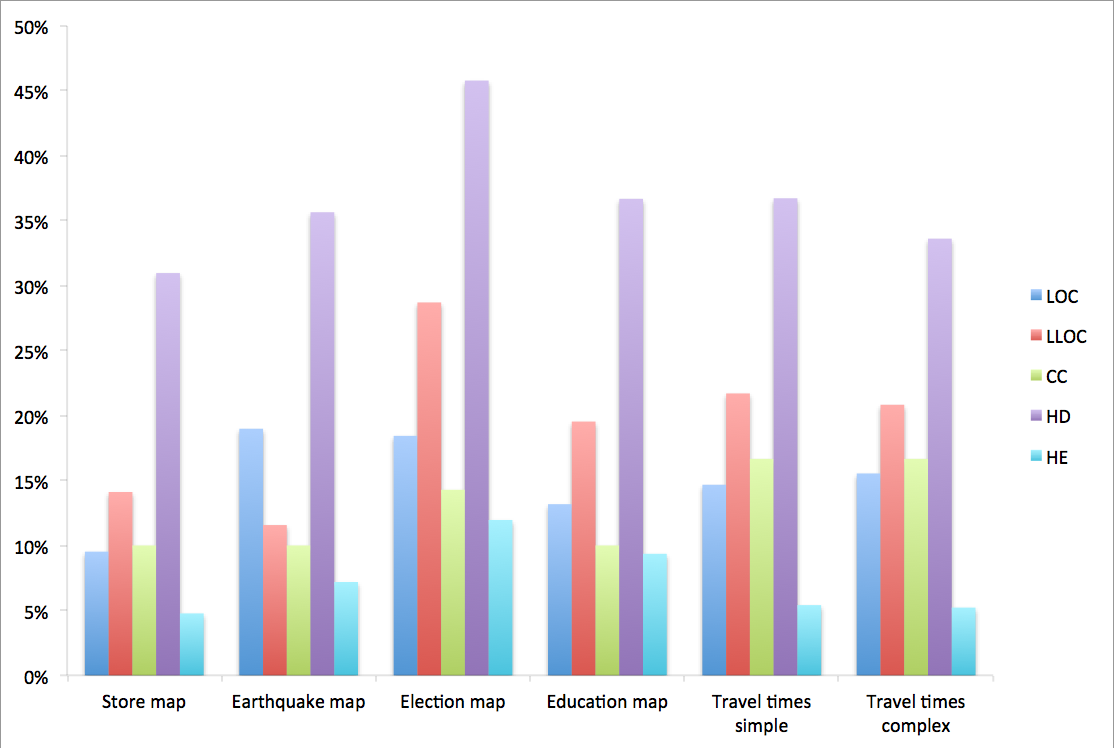
\includegraphics[width=\textwidth]{images/evaluation-results.png}
    \caption{Thematic.js visualization metrics for each case in relation to a corresponding reference visualization. \fixme{Is this the correct way of saying ``metric value in Thematic.js visualization / metric value in reference visualization''?} \fixme{Polish the chart}}
    \label{fig:evaluationchart}
  \end{center}
\end{figure}


According to the results, using Thematic.js yields significantly lower complexity, difficulty and effort values when compared to using no visualization library. This is likely a direct result of Thematic.js providing an extensive map-specific visualization functionality, allowing the visualizer to concentrate on the visualized data. In practice, this means that when creating map visualizations, it is significantly more effective to use a library such as Thematic.js than to write the visualization from the ground up, given that the visualizer possesses -- or is able to achieve -- a general knowledge of the library functionality.

\fixme{Go through all evaluation cases in detail here - describe results and discuss why the results are as they are.}

However, it is likely that the results do not describe the most typical real-life scenarios completely accurately. It can be assumed that typically, visualizers do not possess knowledge of Thematic.js functionality beforehand and therefore effort for each line of code is considerably higher than when building the visualization from the ground up. In the results, this is reflected in high values for relative difficulty as seen in figure \ref{fig:evaluationchart}.

\fixme{Qualitative analysis - don't repeat yourself etc.}

The results of the evaluation are presented in more detail in appendix \ref{appendix:escomplex}.

\section{Evaluating Effectiveness of Visualizations}

\begin{itemize}
	\item Principles by \citet{tufte_visual_1986} (data ink, dont distort, etc.)
	\item Truthfulness by \citet{azzam_j-b_2013}
	\item Guidelines in \citet{kraak_cartographic_1998} (how do i say what to whom and is it effective)
\end{itemize}

You have done your work, but that's\footnote{By the way, do \emph{not} use
shorthands like this in your text! It is not professional! Always write out all
the words: ``that is''.} not enough. 

You also need to evaluate how well your implementation works.  The
nature of the evaluation depends on your problem, your method, and
your implementation that are all described in the thesis before this
chapter.  If you have created a program for exact-text matching, then
you measure how long it takes for your implementation to search for
different patterns, and compare it against the implementation that was
used before.  If you have designed a process for managing software
projects, you perhaps interview people working with a waterfall-style
management process, have them adapt your management process, and
interview them again after they have worked with your process for some
time. See what's changed.

The important thing is that you can evaluate your success somehow.
Remember that you do not have to succeed in making something spectacular; a
total implementation failure may still give grounds for a very good master's
thesis---if you can analyze what went wrong and what should have been done.

 
